
\textbf{Organisationsgrenzen}

\begin{itemize}
    \item \textcolor{blue}{Organisationsintern} Enterprise Architecture Integration (EAI)
    \item \textcolor{blue}{Organisationsübergreifend} B2x, B2B = Business to Business (Lieferanten, Logistikpartner, Finanzinstitute), B2C = Business to Consumer, B2A = Business to Administration (Behörden, Steuerämter, Zoll), E-Business: \\
    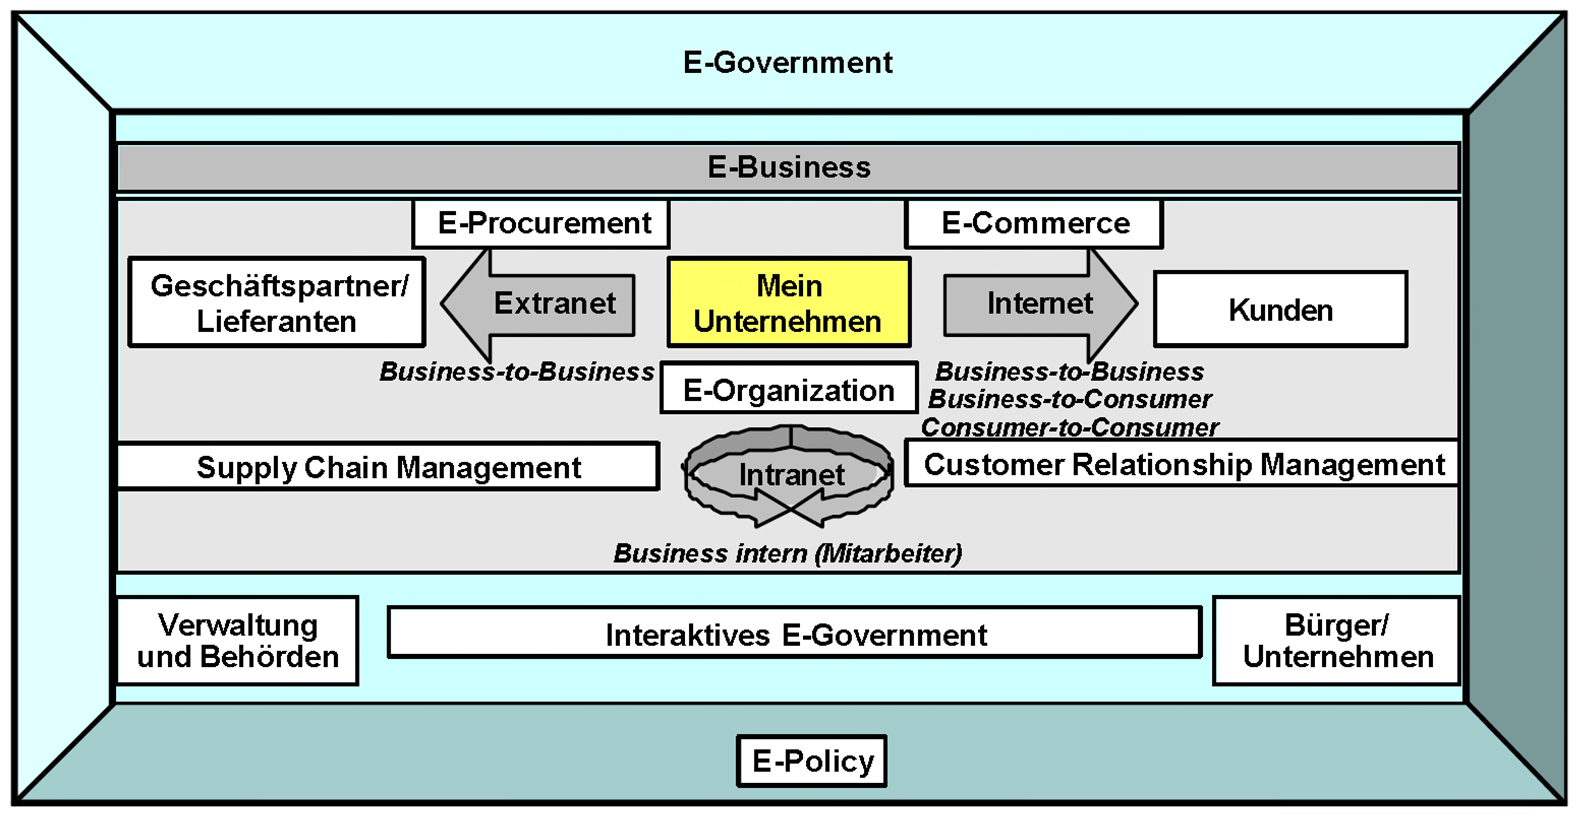
\includegraphics[width=\linewidth]{integration-e-business.png}
\end{itemize}
\vspace{10pt}
\textbf{MSP (Managed Service Provider)}

Cloud Service Intermediäre, der Vorteil für den Kunden ist, dass er technisch nur eine Schnittstelle unterhalten muss. Über Adresse und Wahl des Messagetyps werden Geschäftspartner angesteuert

\begin{itemize}
    \item \textcolor{blue}{Identity SP} Identity Broker, Self-Service, Passwort Management, Single-Sign-on (SSO), Identity und Access Governance \\ $\rightarrow$ Facebook, Google, auth0
    \item \textcolor{blue}{EDI SP} Integration mit EDICFACT, ebXML, CXML, xRechnung usw. \\ $\rightarrow$ Mulesoft, SAP Ariba, Seeburger
    \item \textcolor{blue}{Message SP} einheitliche Schnittstelle für E-Mail, SMS, MMS, WhatsApp, RCS (Rich Communication Services) und Sprachnachrichten \\ $\rightarrow$ - twilio, MessageBird
    \item \textcolor{blue}{Payment SP} Einheitliche Schnittstelle für Zahlungsinstitute, Kreditkarten, Debitkarten, weitere elektronische Zahlungsmittel \\ $\rightarrow$ Payrexx, Stripe
    \item \textcolor{blue}{Karten/Geodaten SP} Landkartendienst \\ $\rightarrow$ Google Maps
    \item \textcolor{blue}{Daten SP} Datendienst wie Adress-, Markt-, Statistik-Daten \\ $\rightarrow$ Finanzinformationen von Six-Group, Open Data Swiss
\end{itemize}
